\LARGE{ \textbf {Лекция №4}}\\
\Large{ \textbf {Нормальные формы булевых функция.}}\\
Аксиомы и основный тождества булевой алгебры логики.\\
Законы де Моргона\\
$
x_1 + x_2 =  \overline{  \overline{x_1} \cdot \overline{x_2 } }\\
x_1 \cdot x_2 =  \overline{  \overline{x_1} + \overline{x_2 } }\\
$
Двойственная формулировка.\\
$
\overline{ x_1 \cdot x_2} = \overline{x_1} + \overline{x_2}\\
\overline{ x_1 + x_2}     = \overline{x_1} \cdot \overline{x_2}\\
$
Справедливы и для $n$ перменных.\\
$
f(a,b,c) = a\overline{b} + ab\overline{c} + \overline{a}\overline{b} \mbox{  --- Дизъюнктивная нормальная форма}\\
f(a,b,c) = (\overline{a} + \overline{b} + c) \cdot (a + \overline{b}) \cdot (\overline{a} + c)  \mbox{  --- Конъюнктивная нормальная форма}\\
f(a,b,c) = abc + a\overline{b}c + \overline{a}b\overline{c} + \overline{a}\overline{b}c  \mbox{  ---Совершенная дизъюнктивная нормальная форма}\\
f(a,b,c) = (a+b+\overline{с}) \cdot (\overline{a}+\overline{b}+c) \cdot (a+\overline{b}+\overline{c})  \mbox{  ---Совершенная конъюнктивная нормальная форма}\\
$
0 - наименьший дизъюнктивный терм.\\
1 - минимальный коньюктивный терм. \\
Минтерм - входят все переменные функции перемножаясь.\\
Макстерм - входят все переменные функции складываясь.\\
Совершенная форма даёт единственно однозначное представление о функции. совершенная форма имеет только 2 вида СКНФ И СДНФ.\\
Любую логическую функцию можно привезти к КНФ И ДНФ используя для преобразования законы булевой алгебры.\\

\Large{ \textbf {Синтез комбинационных схем}}\\
Алгоритм построения совершенных форм по таблице истинности.\\
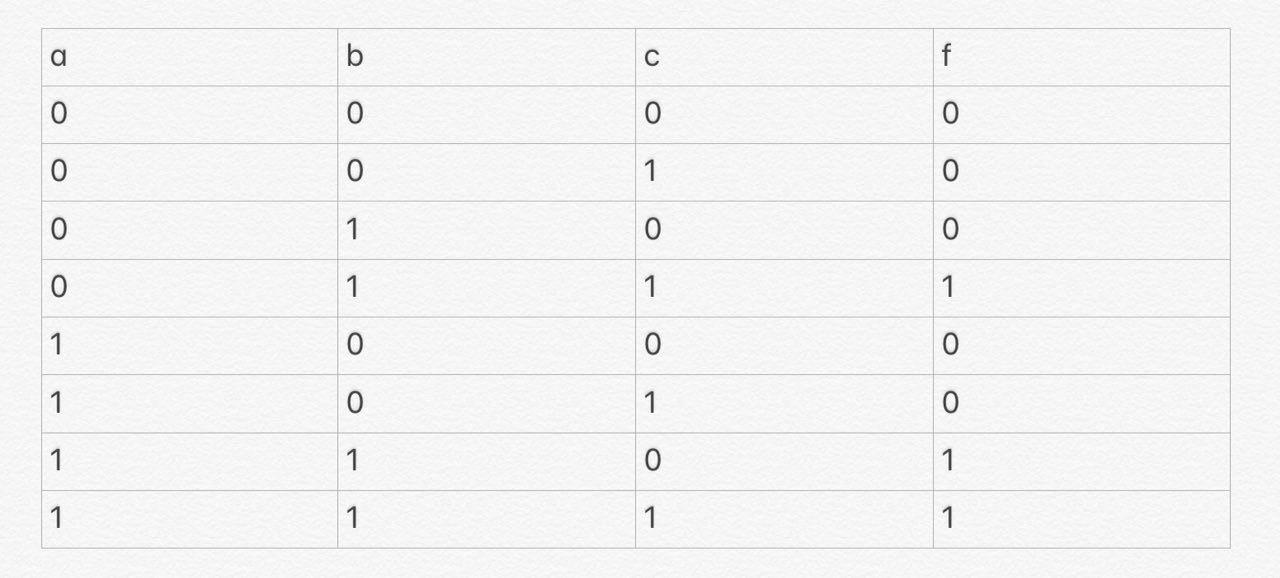
\includegraphics[width=\linewidth]{7}
\Large{ \textbf {Алгоритм построения СДНФ.}}
\begin{enumerate}
  \item Из таблицы выбираются строки, где функция принимает единицу.
  \item Каждой такой строке сопоставляется минтерм, в который переменная входит с отрицанием, если переменная равна 0.
  \item Затем все термы складываются.
\end{enumerate}
Существует двойственный алгоритм получения СКНФ
\begin{enumerate}
  \item Выбираются строки функция равна 0
  \item Каждой строке соответствует макстерм, в который переменная входит с отрицанием, если переменная равна 1.
  \item Затем все перемножается.
\end{enumerate}

Аналитическое представление позволяет описать структуру, а не только поведение.\\
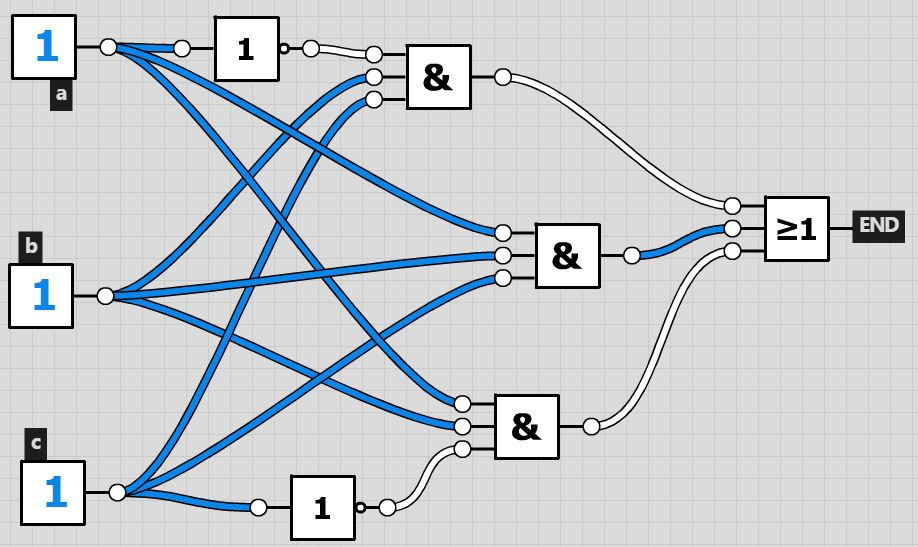
\includegraphics[width=\linewidth]{8}
$
y = \overline{a}bc + ab\overline{c} + abc\\
= \overline{a}bc + ab(\overline{c}+c)\\
= \overline{a}bc + ab\\
=(a + \overline{a}c)b\\
=ab + bc\\
=b(a + c)\\
$
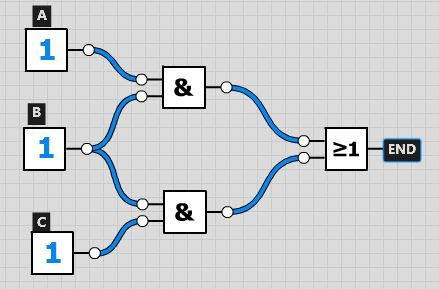
\includegraphics[width=\linewidth/2]{9}
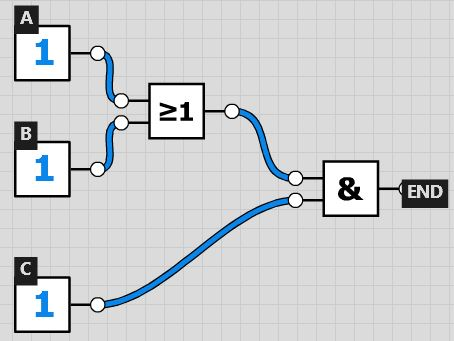
\includegraphics[width=\linewidth/2]{10}
$
\mbox{Трюк:\quad} x_2x_3 = \overline{x_1}x_2x_3 + x_1x_2x_3\\
y = x_1x_2 + x_2x_3 + \overline{x_2}x_3\\
= x_1x_2 + x_1x_2x_3 + \overline{x_1}x_2x_3 + \overline{x_1}x_3\\
= x_1x_2(1 + x_3)  + \overline{x_1}x_3(1 + x_2)\\
=x_1x_2 + \overline{x_1}x_3\\
$

Свойство латентности схем.\\
Аналогичным способом можно построить СКНФ.\\
Получение совершенных форм из произвольных нормальных форм.\\
Произвольная ДНФ приводится К СДНФ.\\
\begin{enumerate}
  \item Пусть в ДНФ есть терм $p$ входящий в функцию от $n$ переменных, не содержит $X_i$
  \item Тогда: $p = p +1 = p(X_i + -X_i)$
\end{enumerate}
Если в дизконъюнктивном терме $q$ отсутсвует $X_j$ :\\
$q = q+ 0= q +X_j + \overline{X_j} =( q+ X_j) (q + \overline{Xj})$\\


\Large{ \textbf {Минимизация логических функций.}}\\
Сложность логической функции в СДНФ и СКНФ, а следовательно и сложность реализующей ее схемы пропорционально числу операций и числу переменных.
Поэтому при проектировании логических схем выполняется минимизация логических функций,
приводящая к минимальным затратам оборудования при аппаратной реализации.\\
Минимизаций логической функции называют нахождение наиболее ее простого представления в смысле минимального числа символов.\\
с помощью законов алгебры логики: склеивание и поглощение\\
пример 3\\
Первый способ имеет недостаток - непонятно какой закон применять, какое тождество использовать для минимизации.\\
Минимизация булевых функций с помощью карт Карно.\\
Похожий метод с диаграммы веича удобен, если функция содержит не более 5-6 логических переменных.\\
Предсляет собой графическое представление таблицы истинности, двухмерное представление.\\
В карно записываются как по горизонтали так и по вертикали.\\

Таблица карты карно делится на квадраты. Если число переменных четно,
то половину пишут по горизонтали, по вертикали. Если число переменных нечетно,
то по вертикали на одну переменную записывают больше.
Порядок размещения значений переменных выбирается в коде Грея.

Примечание:\\
Пусть дано двоичное число $b$, $n$ разрядное, ему можно сопоставить код грея, с тем же разрядом.\\
$Q_n = B_n$\\
$Q_i = B_i +(M2) B_i + 1$\\
Любые 2 соседних числа в коде Грея отличаются одним разрядом.\\
В полученные квадраты заносятся значение функции для соответствующих наборов переменных.\\
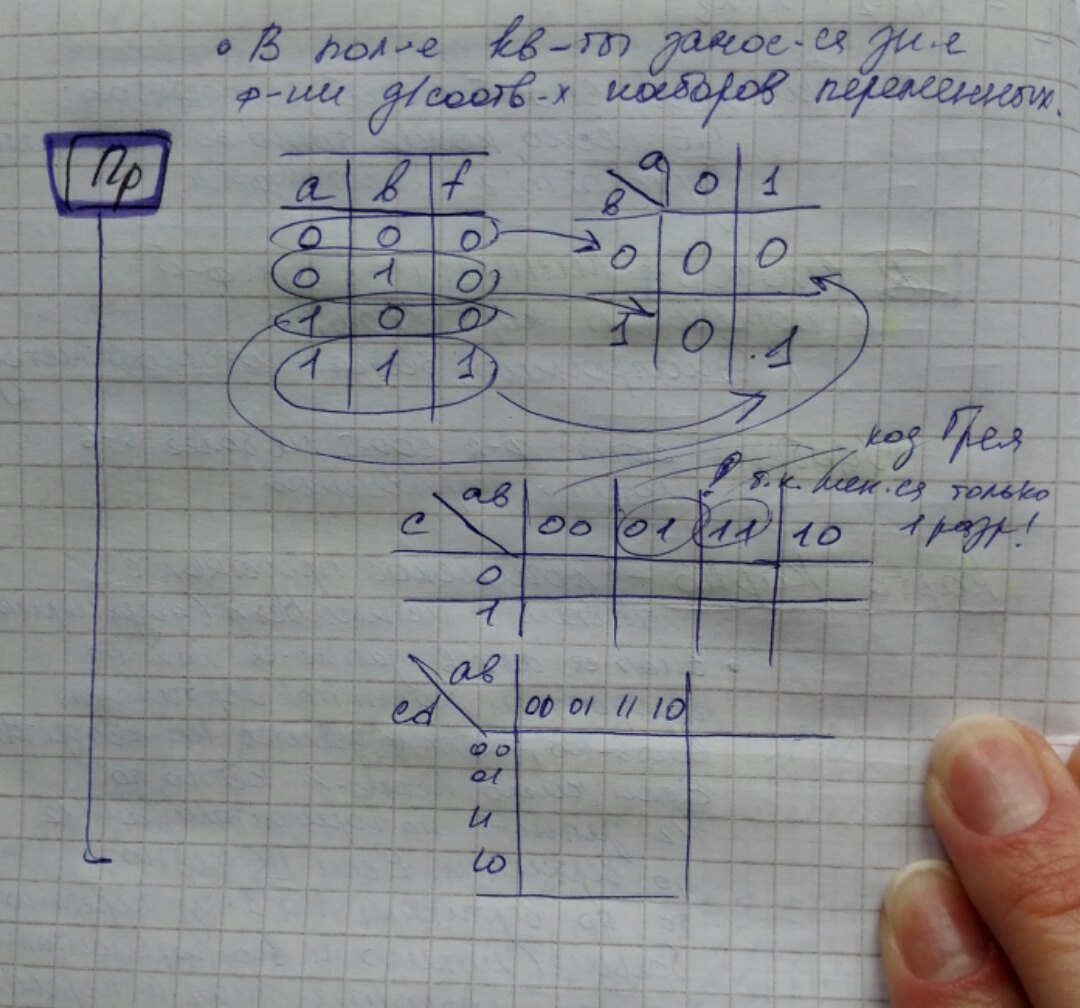
\includegraphics[width=\linewidth]{11}
